\documentclass[12pt, a4paper]{article}

\usepackage[hidelinks]{hyperref}
\usepackage[tmargin=1in, bmargin=1in]{geometry}
\usepackage{parskip}
\usepackage{amssymb}
\usepackage{amsmath}
\usepackage[shortlabels]{enumitem}
\usepackage[dutch]{babel}
\selectlanguage{dutch}
\usepackage{pgfplots}
\pgfplotsset{width=7.5cm, compat=1.18}
\usepackage{amsthm}

\begin{document}

\title{Lineare Algebra - Inleveropgave 1}
\author{Brechtje Poppen - Lotte Gritter - Boris van Boxtel}
\date{23 september 2022 - Week 38} 

\maketitle
\pagenumbering{gobble}

\begin{enumerate}[(a).]
    \item \label{opdrachta}
    Stel $z^n = 1$ met $z \in \mathbb{C}$ en $n \in \mathbb{N}$. Dan is $z$ als volgt te schrijven: $z = re^{i\phi}$, dus $z^n = r^ne^{in\phi} = 1$.

    Voor twee willekeurige getallen $w_1,w_2 \in \mathbb{C}$ met $w_1 = w_2$ geldt $|w_1|=|w_2|$ en  $\text{arg($w_1$)} = \text{arg($w_2$)}$, dus:
    \begin{equation}
        \begin{split}
            |z^n| &= |1| \\
            \text{arg}(z) &= \text{arg}(1)
        \end{split}
    \end{equation}
    We weten dat $|z^n| = r^n$, dus $r^n = 1$, en omdat $r \in \mathbb{R}$, $r = 1$. Ook geldt dat arg($z$) $= in\phi$ en arg(1) = $2k\pi$ met $k \in \mathbb{N}$, dus $n\phi = 2k\pi$. Hieruit volgt dat $\phi = \frac{2k\pi}{n}$.

    Voor een willekeurige $n \in \mathbb{N}$ geldt $r = 1$ en $\phi = \frac{2k\pi i}{n}$. Hieruit volgt dat $z = e^{\frac{2k\pi i}{n}}$. Voor $n = 3$ en $n = 6$ krijg je de volgende eenheidswortels:

    \begin{center}
        \begin{tabular}{c c}
        \begin{tabular}{c|c}
            \multicolumn{2}{c}{$n = 3$} \\
            $k$ & $z$ \\
            \hline
            0 & $1$ \\
            1 & $e^{2\pi i/3}$ \\
            2 & $e^{4\pi i/3}$ \\
        \end{tabular}
        &
        \begin{tabular}{c|c}
            \multicolumn{2}{c}{$n = 6$} \\
            $k$ & $z$ \\
            \hline
            0 & $1$ \\
            1 & $e^{\pi i/3}$ \\
            2 & $e^{2\pi i/3}$ \\
            3 & $e^{\pi i}$ \\
            4 & $e^{4\pi i/3}$ \\
            5 & $e^{5\pi i/3}$ \\
        \end{tabular}
        \end{tabular}
    \end{center}
    \bigskip
    \begin{center}
        \begin{tabular}{c c}
            $n = 3$ & $n = 6$\\
            \begin{tikzpicture}
                \begin{axis}[
                    font=\small,
                    xmin=-1.5,
                    xmax=1.5,
                    ymin=-1.5,
                    ymax=1.5,
                    axis equal,
                    axis lines=middle,
                    xlabel=Re($z$),
                    ylabel=Im($z$),
                    ]
                    \fill [red] ({cos(0)},{(sin(0))}) circle (2pt);
                    \node [anchor=south] at ({cos(0) - 0.2},{(sin(0))}) {$z = 1$};

                    \fill [red] ({cos(1 * 360/3)},{(sin(1 * 360/3))}) circle (2pt);
                    \node [anchor=east] at ({cos(1 * 360/3)},{(sin(1 * 360/3))}) {$z = e^{2\pi i/3}$};

                    \fill [red] ({cos(2 * 360/3)},{(sin(2 * 360/3))}) circle (2pt);
                    \node [anchor=east] at ({cos(2 * 360/3)},{(sin(2 * 360/3))}) {$z = e^{4\pi i/3}$};
                \end{axis}
            \end{tikzpicture}
            &
            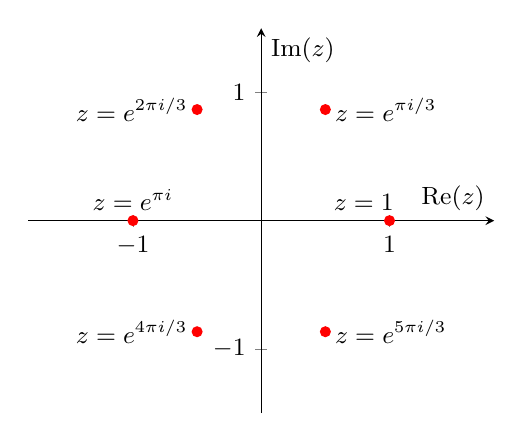
\begin{tikzpicture}
                \begin{axis}[
                    font=\small,
                    xmin=-1.5,
                    xmax=1.5,
                    ymin=-1.5,
                    ymax=1.5,
                    axis equal,
                    axis lines=middle,
                    xlabel=Re($z$),
                    ylabel=Im($z$),
                    ]
                    \fill [red] ({cos(0)},{(sin(0))}) circle (2pt);
                    \node [anchor=south] at ({cos(0) - 0.2},{(sin(0))}) {$z = 1$};

                    \fill [red] ({cos(1 * 360/6)},{(sin(1 * 360/6))}) circle (2pt);
                    \node [anchor=west] at ({cos(1 * 360/6)},{(sin(1 * 360/6))}) {$z = e^{\pi i/3}$};

                    \fill [red] ({cos(2 * 180/3)},{(sin(2 * 180/3))}) circle (2pt);
                    \node [anchor=east] at ({cos(2 * 180/3)},{(sin(2 * 180/3))}) {$z = e^{2\pi i/3}$};

                    \fill [red] ({cos(3 * 180/3)},{(sin(3 * 180/3))}) circle (2pt);
                    \node [anchor=south] at ({cos(3 * 180/3)},{(sin(3 * 180/3))}) {$z = e^{\pi i}$};

                    \fill [red] ({cos(4 * 180/3)},{(sin(4 * 180/3))}) circle (2pt);
                    \node [anchor=east] at ({cos(4 * 180/3)},{(sin(4 * 180/3))}) {$z = e^{4\pi i/3}$};

                    \fill [red] ({cos(5 * 180/3)},{(sin(5 * 180/3))}) circle (2pt);
                    \node [anchor=west] at ({cos(5 * 180/3)},{(sin(5 * 180/3))}) {$z = e^{5\pi i/3}$};
                \end{axis}
            \end{tikzpicture}
        \end{tabular}
    \end{center}
    \newpage
    De som van de n n-de eenheidswortels is 0, omdat alle vectoren opgeteld elkaar opheffen. Voor elke n is 1 een eenheidswortel. Wanneer $n$ even is, zoals bij $n = 6$, heffen alle getallen met een complex deel niet gelijk aan 0 elkaar op, en blijven alleen -1 en 1 over, die elkaar vervolgens opheffen. Wanneer $n$ oneven is, is de som van alle getallen waarvan het complexe deel niet gelijk is aan nul, -1. Deze heft vervolgens de overgebleven eenheidswortel met waarde 1 op.
    
    Voorbeelden:
       \begin{center}
        $n = 6$
    \end{center}
    \begin{center}
        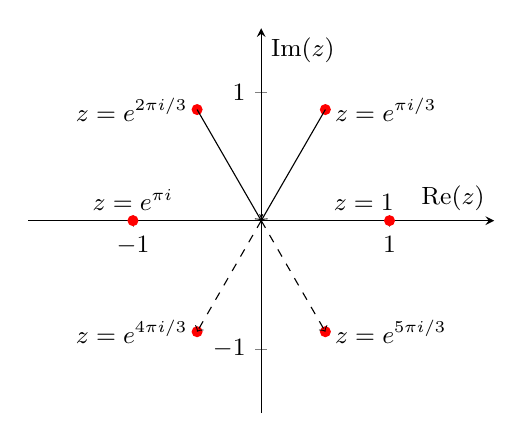
\begin{tikzpicture}
            \begin{axis}[
                font=\small,
                xmin=-1.5,
                xmax=1.5,
                ymin=-1.5,
                ymax=1.5,
                axis equal,
                axis lines=middle,
                xlabel=Re($z$),
                ylabel=Im($z$),
                ]
                \fill [red] ({cos(0)},{(sin(0))}) circle (2pt);
                \node [anchor=south] at ({cos(0) - 0.2},{(sin(0))}) {$z = 1$};

                \fill [red] ({cos(1 * 360/6)},{(sin(1 * 360/6))}) circle (2pt);
                \node [anchor=west] at ({cos(1 * 360/6)},{(sin(1 * 360/6))}) {$z = e^{\pi i/3}$};

                \fill [red] ({cos(2 * 180/3)},{(sin(2 * 180/3))}) circle (2pt);
                \node [anchor=east] at ({cos(2 * 180/3)},{(sin(2 * 180/3))}) {$z = e^{2\pi i/3}$};

                \fill [red] ({cos(3 * 180/3)},{(sin(3 * 180/3))}) circle (2pt);
                \node [anchor=south] at ({cos(3 * 180/3)},{(sin(3 * 180/3))}) {$z = e^{\pi i}$};

                \fill [red] ({cos(4 * 180/3)},{(sin(4 * 180/3))}) circle (2pt);
                \node [anchor=east] at ({cos(4 * 180/3)},{(sin(4 * 180/3))}) {$z = e^{4\pi i/3}$};

                \fill [red] ({cos(5 * 180/3)},{(sin(5 * 180/3))}) circle (2pt);
                \node [anchor=west] at ({cos(5 * 180/3)},{(sin(5 * 180/3))}) {$z = e^{5\pi i/3}$};

                \draw[dashed, ->] (0,0) -- ({cos(4 * 180/3)},{(sin(4 * 180/3))});
                \draw[dashed, ->] (0,0) -- ({cos(5 * 180/3)},{(sin(5 * 180/3))});

                \draw[->] ({cos(1 * 180/3)},{(sin(1 * 180/3))}) -- (0,0);
                \draw[->] ({cos(2 * 180/3)},{(sin(2 * 180/3))}) -- (0,0);
            \end{axis}
        \end{tikzpicture}
    \end{center}
    \begin{center}
        \footnotesize We zien hier dat de som van de complexe getallen die niet op de reële as liggen 0 is, en vervolgens -1 en 1 overblijven. Deze twee heffen elkaar op, en dus houden we 0 over.
    \end{center}
    \begin{center}
        $n = 3$
    \end{center}
    \begin{center}
        \begin{tikzpicture}
            \begin{axis}[
                font=\small,
                xmin=-1.5,
                xmax=1.5,
                ymin=-1.5,
                ymax=1.5,
                axis equal,
                axis lines=middle,
                xlabel=Re($z$),
                ylabel=Im($z$),
                ]

                \fill [red] ({cos(0)},{(sin(0))}) circle (2pt);
                \node [anchor=south] at ({cos(0) - 0.2},{(sin(0))}) {$z = 1$};

                \fill [red] ({cos(1 * 360/3)},{(sin(1 * 360/3))}) circle (2pt);
                \node [anchor=east] at ({cos(1 * 360/3)},{(sin(1 * 360/3))}) {$z = e^{2\pi i/3}$};

                \fill [red] ({cos(2 * 360/3)},{(sin(2 * 360/3))}) circle (2pt);
                \node [anchor=east] at ({cos(2 * 360/3)},{(sin(2 * 360/3))}) {$z = e^{4\pi i/3}$};

                \draw[dashed, ->] (0,0) -- ({cos(2 * 360/3)},{(sin(2 * 360/3))});
                \draw[->] (0,0) -- ({cos(1 * 360/3)},{(sin(1 * 360/3))});
                \draw[->] ({cos(1 * 360/3)},{(sin(1 * 360/3))}) -- (-1,0);
            \end{axis}
        \end{tikzpicture}
    \end{center}
    \begin{center}
        \footnotesize We zien hier dat de som van de twee complexe getallen behalve 1, samen opgeteld -1 zijn. Dit heft op met de overgebleven eenheidswortel 1, en dus houden we 0 over.        
    \end{center}
    \bigskip
    \item 
    De n-de eenheidswortels zijn $z = e^{\frac{2k\pi i}{n}}$ met $k \in \mathbb{N}$. Zie opdracht \ref{opdrachta} voor de afleiding hiervan.

    De n-de eenheidswortels zijn weer te geven in het complexe vlak als punten die gelijkmatig zijn verdeeld over de eenheidscirkel. Er zijn altijd n aantal eenheidswortels. De hoek tussen twee opeenvolgende eenheidswortels is altijd $\frac{2\pi}{n}$.

    \item 
    Neem $\omega = e^{\frac{2\pi i}{n}}$ de eenheidswortel met het kleinste positieve argument, dan zijn de overige eenheidswortels te schrijven als $\omega^k$ voor een $k \in \mathbb{N}$, want ${(e^{\frac{2\pi i}{n}})}^k = e^{\frac{2k\pi i}{n}}$ is de algemene vorm van de eenheidswortels.
    \newpage
    \item \label{opdrachtd}
    Te bewijzen: $1 + \omega + \omega^2 + \dots + \omega^{n - 1} = 0$.

    \begin{proof}
        $ $\newline
        Neem $S = 1 + \omega + \omega^2 + \dots + \omega^{n - 1}$. \newline
        Dan $S \cdot \omega = \omega + \omega^2 + \dots + \omega^n = S - 1 + \omega^n$. \newline
        Dan kunnen we schrijven $S\cdot \omega - S = -1 + \omega^n$. \newline
        Omdat $\omega^n = {(e^{\frac{2\pi i}{n}})}^n = e^{2\pi i} = 1$, $-1 + \omega^n = 0$. \newline
        Dus $S(\omega - 1) = 0$. \newline 
        Omdat $\text{arg(1)}= 0$, en $\omega$ de eenheidswortel is met het kleinste postitieve argument, is $\omega$ niet 1. \newline Hieruit volgt dat $(\omega - 1)$ niet gelijk is aan nul. \newline Dus $S = 1 + \omega + \omega^2 + \dots + \omega^{n - 1} = 0$.
    \end{proof}

    \item 
    Elke term in de som $1 + \omega + \omega^2 + \dots + \omega^{n - 1}$ corrospondeert exact met een eenheidswortel en alle eenheidswortels corrosponderen exact met een term in deze som. Bij \ref{opdrachtd} \!hebben we bewezen dat deze som gelijk is aan 0, dus de som van alle eenheidswortels is 0.
    
    \item 
    De eenheidswortels van $x^3+x^2+x+1$, zijn de oplossingen van de vergelijking $x^3+x^2+x+1=0$ met $x \in \mathbb{C}$.
    Het is duidelijk dat een van de oplossingen is $x=-1$. Dus $(x+1)$ is een factor. Door middel van een staartdeling vinden we dat    $x^3+x^2+x+1=(x+1)(x^2+1)$. Dit kunnen we verder factoriseren naar $(x+1)(x+i)(x-i)$. Hieruit volgt dat $x+1=0$ of $x+i=0$ of $x-i=0$. Dus $x=-1, x=-i$ of $x=i$.
    
    \begin{center}
        \begin{tikzpicture}
                \begin{axis}[
                    font=\small,
                    xmin=-1.5,
                    xmax=1.5,
                    ymin=-1.5,
                    ymax=1.5,
                    axis equal,
                    axis lines=middle,
                    xlabel=Re($z$),
                    ylabel=Im($z$),
                    ]
                    \fill [red] ({cos(180)},{(sin(180))}) circle (2pt);
                    \node [anchor=south] at ({cos(180)},{(sin(180))}) {$z = -1$};

                    \fill [red] ({cos(90)},{(sin(90))}) circle (2pt);
                    \node [anchor=west] at ({cos(90)},{(sin(90))}) {$z = i$};

                    \fill [red] ({cos(-90)},{(sin(-90))}) circle (2pt);
                    \node [anchor=west] at ({cos(-90)},{(sin(-90))}) {$z = -i$};
                \end{axis}
            \end{tikzpicture}
    \end{center}
\end{enumerate}









\end{document}